\chapter{Teorema de Noether para campos}

	
\begin{tikzpicture}
	\fill [left color=red!50, right color=teal!50] (0,0) rectangle (6.5,.1);
	\fill [left color=teal!50, right color=blue!50] (6.5,0) rectangle (11.5,.1);
	\end{tikzpicture}


\vspace{10mm}
\begin{adjustwidth}{50pt}{50pt}
\begin{ejemplo}
En el capítulo anterior consideramos la acción y lagrangiano muy generales:

$$ S[\phi] \ =\  \displaystyle \int \dd^4 x \ \mathcal L(\phi, \partial_\mu \phi) \qquad \qquad  \mathcal L\ = \ \dfrac 1 2  \ \partial_\mu \phi \ \partial^\mu \phi \ - \ U(\phi) $$

Vimos que si el campo y sus derivadas se comportaban bien, se anulaban en el infinito ($\phi,\ \partial_\mu \phi \sim 0 \ \text{ si } \ x\to \infty)$ y si además había una simetría de traslación: $\tilde{x^\mu}=x^\mu+a^\mu (cte)$ en que $\tilde \phi(\tilde x)=\phi(x)$, en esas condiciones había un tensor $T^{\mu \nu}$ de divergencia cero:

$$T^{\mu \nu} \ = \ \displaystyle \pdv{\mathcal L}{(\partial_\mu \phi)} \ \partial^\mu \phi \ - \ g^{\mu \nu} \ \mathcal L \qquad  \qquad \partial_\mu \ T^{\mu \nu} \ = \ 0$$

En este capítulo veremos el caso más general, que cubrirá casi todas las simetrías que nos podamos encontrar, en que la traslación puede no ser constante:

\vspace{-5mm}
$$\begin{cases} \ \centerdot \quad  \tilde x^\mu  \ = \ x^\mu \ + \ \delta x^\mu \\  \ \centerdot \quad  \tilde \phi (\tilde x) \ = \ \phi(x) \ + \ \bar \delta \phi   \end{cases}$$

\vspace{3mm}

\end{ejemplo}
\end{adjustwidth}

\vspace{5mm}
\section{Teorema de Noether para campos}

Empecemos con un ejemplo. Consideremos la siguiente acción sencilla (para ver esto del $\bar \delta \phi$):

$$\boldsymbol{ S[\phi] \ = \ \displaystyle \int \dd^4 x\ \dfrac 1 2 \ \partial_\mu \phi \ \partial^\mu \phi^*}$$

Donde $ \phi^* \ $  es el conjugado del campo $\ \phi \, , \  $  es decir, $\ \phi \in \mathbb C$


\begin{figure}[H]
	\centering
	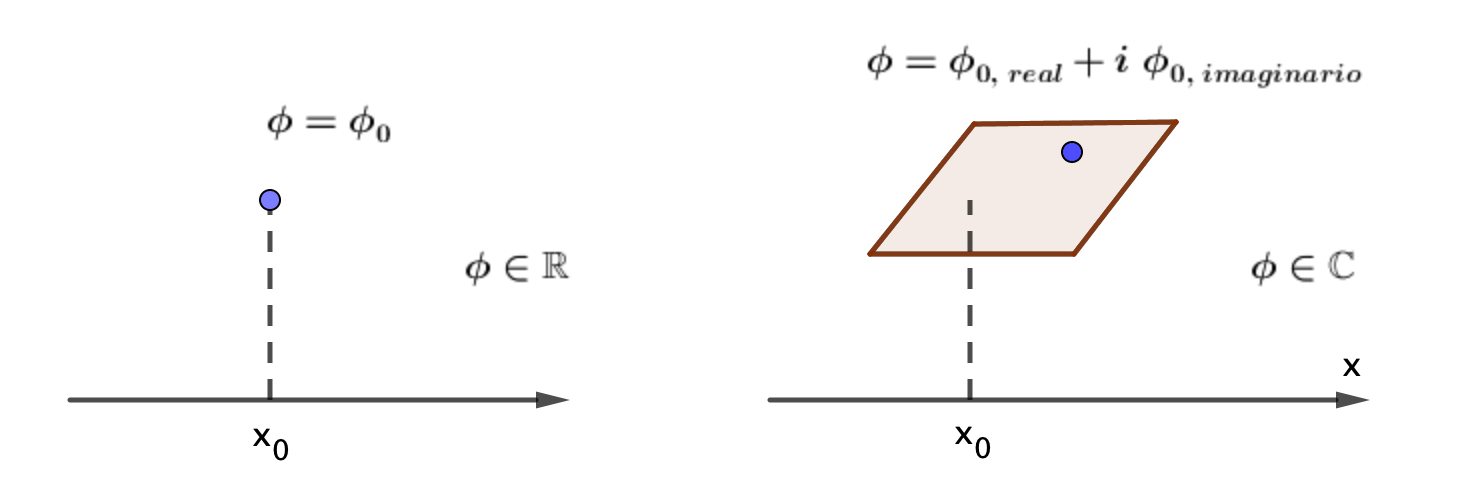
\includegraphics[width=.75\textwidth]{imagenes/img35-01.png}
\end{figure}

El hecho de  multiplicar $\partial_\mu \phi$ por $\partial^\mu \phi^*$ asegura que la acción es real, como debe ser: $S[\phi] \in \mathbb R$

\color{gris}
\underline{Ejemplo}: 

\vspace{-5mm}
\hspace{2 cm} $\phi=e^{-x^2}+i\cos x \to \phi'=-2xe^{-x^2}+i\sin x;\quad \phi^*=e^{-x^2}-i\cos x \to {\phi^*}'=-2xe^{-x^2}-i\sin x$

\hspace{2 cm} $\phi \phi^*=(-2xe^{-x^2}+i\sin x)(-2xe^{-x^2}-i\sin x)=(a+bi)(a-bi)=a^2+b^2\in \mathbb R$ \hspace{2.5cm}$\Box$

\color{black}

\vspace{5mm} Este campo tiene una \emph{simetría continua \textbf{`interna'}}, que no ocurre en el espacio real sino en el plano complejo que hemos asociado a cada puntos del espacio tiempo (figura anterior):

$$\text{simetría continua \emph{interna}}:\qquad \qquad \boldsymbol{ \tilde  \phi \ = \ e^{ib} \ \phi } \, , \qquad b\in \mathbb R$$

Veamos que esta simetría interna deja invariante la acción:


\hspace{1cm} $\partial_\mu \tilde \phi=e^{ib} \partial_\mu \phi\quad \textcolor{gris}{(b=cte)} \qquad \tilde \phi=e^{-ib} \phi \ \to \  \partial_\mu \tilde \phi^*=e^{-ib}\partial_\mu \phi^*$

\hspace{1cm} Para subir el índice, $\ g^{\alpha \mu}\partial\-\mu \tilde \phi^* = g^{\alpha \mu} e^{-ib} \partial_\mu \phi^* \ \to \ \partial^\alpha \tilde \phi^* = e^{-ib} \partial^\mu \phi^*$

\hspace{1cm} Con ello, $\ \partial_\mu \tilde \phi \ \partial^\mu \tilde \phi^*=e^{ib} \partial_\mu \phi \ e^{-ib} \partial^\mu \phi^*=\partial_\mu \phi \partial^\mu \phi^*$ 
\hspace{1cm} y la acción queda invariante $\qquad \ \ \Box$

\vspace{5mm}
\begin{multicols}{2}
\underline{Simetría continua interna}:

$\quad$ --- continua: $\ \ b\in \mathbb R:\ \ b \to 0 \ \Rightarrow \  \tilde \phi \approx \phi$

$\quad$ --- interna: el multiplicar por $e^{ib}$ es como una \emph{rotación} de ángulo $b$ en el espacio interno complejo asociado a cada punto espacio temporal.

\begin{figure}[H]
	\centering
	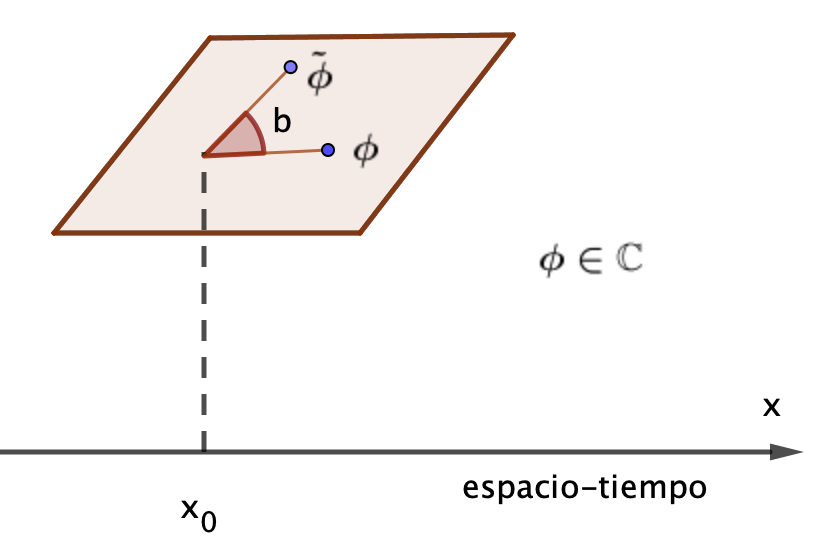
\includegraphics[width=.4\textwidth]{imagenes/img35-02.png}
\end{figure}
\end{multicols}

Además, tenemos una \underline{simetría de traslación}: $\ \tilde x^\mu=x^\mu+a^\mu (cte) \ \to \ \partial_{\tilde \mu}=\partial_\mu + 0 (cte)$ y la acción es \emph{invariante} bajo esta \emph{traslación espacio temporal} (como ya vimos en el capítulo anterior). 


$\triangleright \quad$ Veamos como cambia el campo bajo estas transformaciones:
$\ \  \tilde \phi(\tilde x)=e^{ib} \phi(\tilde x) = e^{ib} \phi(x^\mu+a^\mu)\ $, con $\ a^\mu\ / \ (a^\mu)^2\approx 0 \ \text{ y } \ b\ /\ b^2\approx 0\, , \ $ ambas transformaciones infinitesimales.

Quedándonos a primer orden en el desarrollo de Taylor, $\ \phi(x^\mu + a^\mu) \approx \phi(x\mu)+a^\mu \partial_\mu \phi \ $ y, por otra parte, $\ e^{ib} \approx 1+ib\ $ con lo que:

$\tilde \phi(\tilde x)\approx (1+ib)(\phi(x^\mu)+a^\mu \delta_\mu \phi)=
\phi(x^\mu)+a^\mu \partial_\mu \phi+ ib \phi(x^\mu)+i \cancelto{0}{b a^\mu} \partial_\mu \phi=\phi(x^\mu)+a^\mu \partial_\mu \phi+ ib \phi(x^\mu)$


Llamamos $\quad \boldsymbol{\bar \delta \phi} \ = \ \tilde \phi(\tilde x) \ - \ \phi(x) \ = \ ib \phi(x) \ + \ a^\mu \partial_\mu \phi \qquad (1)$

Pero, $\quad \bar \delta \phi= \tilde \phi(\tilde x) -\phi(x)=\tilde \phi(x^\mu+a^\mu)-\phi(x)= \tilde \phi(x^\mu)+a^\mu \partial_\mu \phi - \phi(x)= \underbrace{ \tilde \phi(x^\mu)-\phi(x) }_{\delta \phi} + a^\mu \partial_\mu \phi$

Luego, $\quad \boldsymbol{ \bar \delta \phi}=\delta \phi +a^\mu \partial_\mu \phi \qquad (2)$

De los resultados $(1)$ y $(2)\, : \qquad \delta \phi \ + \ \cancel{ a^\mu \partial_\mu \phi} \  \approx \  ib \phi \ +\ \cancel{ a^\mu \partial_\mu \phi}$

Conclusión: $\qquad \qquad \boldsymbol{\bar \delta \phi \ \approx \ \delta \phi \ + \ a^\mu \partial_\mu \phi  \qquad \qquad \qquad \delta \phi \ \approx \ ib\phi }$

\vspace{5mm} Si en lugar de $a^\mu$ ponemos una variación genérica $\delta x^\mu$, de modo que la traslación sea $\tilde x^\mu = x^\mu+\delta x^\mu$, en este caso tendremos: $\quad \boldsymbol{\bar \delta \phi \ \approx \ \delta \phi \ + \ \delta x^\mu \ \partial_\mu \phi}$

Resumiendo:

\begin{table}[H]
\center
\begin{tabular}{lll}
$\tilde x^\mu = x^\mu+\delta x^\mu$  &  $\qquad$ &  $\bar \delta \phi=\tilde \phi (\tilde x)-\phi(x)$ \\ \\
$\delta \phi=\tilde \phi(x)-\phi(x)$ &  $\qquad$ &  $\bar \delta \phi=\delta \phi+\delta x^\mu \partial_\mu \phi$
\end{tabular}
\end{table}

\vspace{5mm} $\triangleright \quad$ ?`Qué hay del lagrangiano?, ?`cómo se comporta bajo estas simetrías?

$\mathcal L(\phi, \partial_\mu \phi)\, . \ $ En el capítulo anterior vimos $\ \displaystyle (\delta \mathcal L)_{E-L} \ = \ \partial_\mu \left( \pdv{\mathcal L}{(\partial_\mu \phi)} \ \delta \phi \right)$

También en el capítulo anterior, para $\ \delta \phi=-a^\mu \partial_\mu \phi\, , \ $ obtuvimos $\ \delta \mathcal L = -a^\mu \partial_\mu \mathcal L\, . \ $ ?`Ocurrirá lo mismo ahora?, $\ $ ?`$\  \bar \delta \mathcal L = \delta \mathcal L + \delta x^\mu \partial_\mu \mathcal L\ $?

La respuesta es no, porque:

\vspace{-3mm} \hspace{1cm} --- $\mathcal L$ es invariante ante la transformación $\ \tilde x^\mu=x^\mu +\delta x^\mu$

\vspace{-3mm} \hspace{1cm} --- $\mathcal L$ no es invariante ante la transformación $\ \tilde \phi(x)=e^{ib} \phi(x) \ \to \ \tilde {\mathcal L} =e^{ib} \mathcal L  \ \to \ \tilde S \neq S$

$\bar \delta \phi \ \approx \ \delta \phi \ + \ \delta x^\mu \partial_\mu \phi \ \to \ \delta \phi \ \approx \  \bar \delta \phi \ - \ \delta x^\mu \partial_\mu \phi \ \Rightarrow \ \displaystyle (\delta \mathcal L)_{E-L} = \partial_\mu  \left( \pdv{\mathcal L}{(\partial_\mu \phi)} \ 
(\bar \delta \phi - \delta x^\mu \partial_\mu \phi)
 \right)$

Veamos que ocurre con el lagrangiano al variar las dos simetrías: $\tilde x^\mu =x^\mu+\delta x^\mu \ $ y $ \ \tilde \phi(x)=e^{ib}\phi(x)$.

\underline{Simplificando el problema}, para mayor comprensión:

Queremos ver si $\ \displaystyle \int_{\tilde a}^{\tilde b} \tilde f(\tilde x)\dd x=\int_a^b f(x)\dd x \ $ o, de otro modo, $\ \displaystyle \int_{\tilde a}^{\tilde b} \tilde f(\tilde x)\dd x-\int_a^b f(x)\dd x=0$

\vspace{-3mm} \hspace{1cm} ---Llamamos $\ \begin{cases} \ \tilde a = a+\delta a \\ \ \tilde b = b+\delta b \end{cases}\ $ 

\vspace{-3mm} \hspace{1cm} ---Como en la integral primera la variable $\tilde x$ es muda la llamaremos x.

\vspace{-3mm} \hspace{1cm} --- $\tilde f(x)-f(x)=\delta f \ \to \ \tilde f(x)=f(x)+\delta f$

Entones, escribiremos la expresión anterior como:

$\displaystyle \int_{a+\delta a}^{b+\delta b} (f(x)+\delta f) \ \dd x - \int_a^b f(x) \ \dd x=0 \ \to \ \displaystyle \int_{a+\delta a}^{b+\delta b} f(x) \ \dd x 
- \int_a^b f(x) \ \dd x +
\displaystyle \int_{a+\delta a}^{b+\delta b} \delta f \ \dd x=0$

\vspace{5mm}
\begin{multicols}{2}
$\quad$ 

Las áreas de la figura adjunta cumplen:

$$(B+C)-(A+B)=C-A$$

Cada una de ellas, como se trata de `trapecios' de base infinitesimal, valen: 

$$f(b)\delta b \ - \ f(a)\delta a$$

$\quad$ 
\begin{figure}[H]
	\centering
	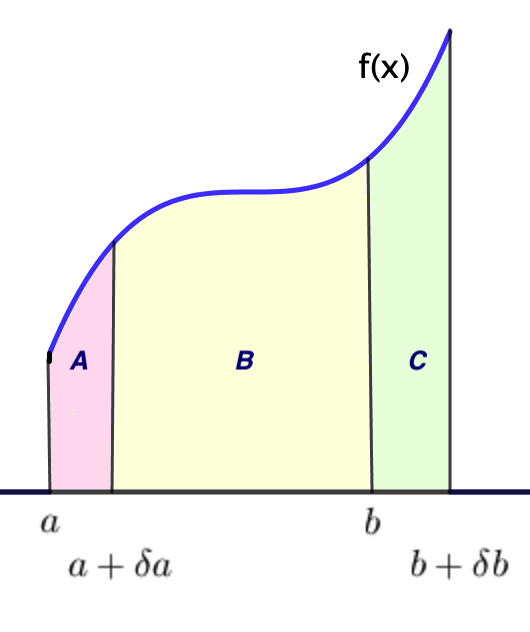
\includegraphics[width=.20\textwidth]{imagenes/img35-03.png}
\end{figure}
\end{multicols}

Así, $\quad \displaystyle \int_{\tilde a}^{\tilde b} \tilde f(\tilde x)\dd x-\int_a^b f(x)\dd x \ = \ f(b)\delta b \ - \ f(a)\delta a + \int_a^b \delta f(x) \ \dd x$

De otro modo, $\quad \displaystyle \eval{f(x)\delta x}_a^b + \int_a^b \delta (f(x) \ \dd x = 0 \ \to \ \int_a^b \dv{x} \left( f(x)\delta x \right) \ \dd x+ \int_a^b f(x)\ \dd x =0$

Es decir, $\quad \displaystyle \int_a^b \left[ \ \dv{x} \left( f(x)\delta x \right) \ + \ \delta f(x) \ \right] \ \dd x \ = \ 0$

\underline{Traduzcamos este resultado a nuestro lagrangiano} (abandonando la simplificación del problema):

$$\displaystyle \boldsymbol{ \int \dd^4 x \ [ \ \delta \mathcal L \ + \ \partial_\mu (\mathcal L \, \delta x^\mu) \ ] \ = \ 0 }$$

Para que la acción quede invariante ante la simetría ha de ocurrir que:

$$\boldsymbol{ \boxed{ \ (\delta \mathcal L)_S \ = \ -\partial_\mu (\mathcal L \, \delta x^\mu) \ } }$$

\textcolor{gris}{En el capítulo anterior obtuvimos $\ (\delta \mathcal L)_S=-a^\mu(cte)\, \partial_\mu \mathcal L =-\partial_\mu (a^\mu \, \mathcal L)\, , \ $ ahora no podemos sacar fuera de $\partial_\mu)$ el factor $\delta x^\mu$ porque no es constante.}

\vspace{5mm}

Ya tenemos todos los elementos preparador para enunciar el teorema e Noether para campos:

$\left.
\begin{matrix} 
(\delta \mathcal L)_{E-L} \ = \ \partial_\mu \displaystyle \left( \pdv{\mathcal L}{(\partial_\mu \phi)} \ ( \underbrace{\bar \delta \phi - \delta x^\alpha \partial_\alpha \phi}_{(\delta \phi)_S}\ ) \right) \ \ \\ \\ (\delta \mathcal L)_S \ = \ -\partial_\mu (\mathcal L \ \delta x^\mu ) \end{matrix} \right\}\ \Rightarrow \ \partial_\mu  \displaystyle \left( \pdv{\mathcal L}{ (\partial_\mu \phi) } \ ( \bar \delta \phi - \delta x^\alpha \partial_\alpha \phi) \right) \ = \ -\partial_\mu (\mathcal L \ \delta x^\mu)$

$\displaystyle 
\partial_\mu  \displaystyle 
\left[\ 
\left( \pdv{\mathcal L}{ (\partial_\mu \phi) } \ ( -\bar \delta \phi + \delta x^\alpha \partial_\alpha \phi) \right) \ - \ \partial_\mu (\mathcal L \ \delta x^\mu)  \ \right] 
\ = \ 0$

$\displaystyle 
\partial_\mu  \displaystyle 
\left[\ 
- \pdv{\mathcal L}{ (\partial_\mu \phi) } \ \bar \delta \phi \ 
+ \pdv{\mathcal L}{ (\partial_\mu \phi) } \ \delta x^\alpha \partial_\alpha \phi
- \mathcal L \ \delta x^\mu  \ \right] 
\ = \ 0$

Como $\quad \delta x^\mu\ =\ \delta_\alpha^\mu \ \delta x^\alpha\, , 	 \ \text{ con } \ \delta_\alpha^\mu \ $ el delta de Kronecker,

$\displaystyle \partial_\mu 
\left[ \ 
-\pdv{\mathcal L}{(\partial_\mu \phi)} \ \bar \delta \phi \ 
+ \ \pdv{\mathcal L}{(\partial_\mu \phi}\ \delta^\alpha \partial_\alpha \phi \ - \ 
\mathcal L \ \delta_\alpha^\mu \ \delta x^\alpha 
\ \right] \ = \ 0$

$\displaystyle \partial_\mu 
\left[ \ 
-\pdv{\mathcal L}{(\partial_\mu \phi)} \ \bar \delta \phi \ + \ 
\delta x^\alpha \ \left(
\underbrace{
\pdv{\mathcal L}{(\partial_\mu \phi)} \ \partial_\alpha \phi \ - \ \mathcal L \ \delta_\alpha^\mu }_{ T^\mu_\alpha \ \text{ cap. anterior}}
\right)
 \ \right]  \ = \ 0$
 

$\displaystyle \partial_\mu \left[ \ -\pdv{\mathcal L}{(\partial_\mu \phi)} \ \bar \delta \phi \ + \ T^\mu_\nu \ \delta x^\nu \ \right] \ = \ 0$

Luego,

\vspace{0.5cm}

\begin{large}
\begin{myblock}{Teorema de Noether para campos}
\vspace{2mm}
\begin{equation}
\label{T35TNC}
\boldsymbol{
\partial_\mu \left[ \ -\pdv{\mathcal L}{(\partial_\mu \phi} \ \bar \delta \phi \ - \ T^\mu_\nu \ \delta x^\nu \ \right] \ = \ 0
}	
\end{equation}
	Aparece el tensor energía momento contraído con las variaciones de $x^\nu$.
	
	Se llama \textbf{cuadrivector corriente} a $\ \boldsymbol{ J^\mu \ = \ \displaystyle  \ -\pdv{\mathcal L}{(\partial_\mu \phi} \ \bar \delta \phi \ - \ T^\mu_\nu \ \delta x^\nu }$
	
	La divergencia del cuadrivector corriente es cero, el cuadrivector corriente se va a conservar.
	
\begin{equation}
\label{T35-4vJ}
\boldsymbol{
\partial_\mu \ J^\mu \ = \ 0
}	
\end{equation}

Teorema de Noether bastante general, cubre muchísimas simetrías.
\vspace{2mm}
\end{myblock}
\end{large}

\vspace{5mm}
\begin{ejemplo}
El término $\displaystyle \  \pdv{\mathcal L}{(\partial_\mu \phi)} \ \bar \delta \phi \, , \  $	bajo determinada simetría, nos dará el spín; como predice la  \emph{teoría cuántica de campos relativista}
\end{ejemplo}





